\chapter{Implementation}


\section{Iterative testing}
\subsection{Testing of alpha version}


\textbf{State of the game:} The game supports controlling with one Myo device. It allows to shoot different colours lasers with different gestures. All asteroids are the same and they response to any kind of color. Backgrounds is an image. Basic UI counts successes and informs about Myo status (synchronized, connected etc.). Game is buggy, has stack overflow problems and allows accumulating not-destroyed asteroids in player's scene view.

\textbf{Testing group:} three male adults, under 30 yo, with supervision of author

\textbf{Testing outcome:} 

\begin{itemize}
\item background and ground should be 3D structures to allow better depth recognition
\item the scene should have better lights
\item making the controls more advanced may result in more interesting game
\item missiles should be faster
\item using two hands for controlling seems to be interesting idea
\end{itemize}
\begin{figure}
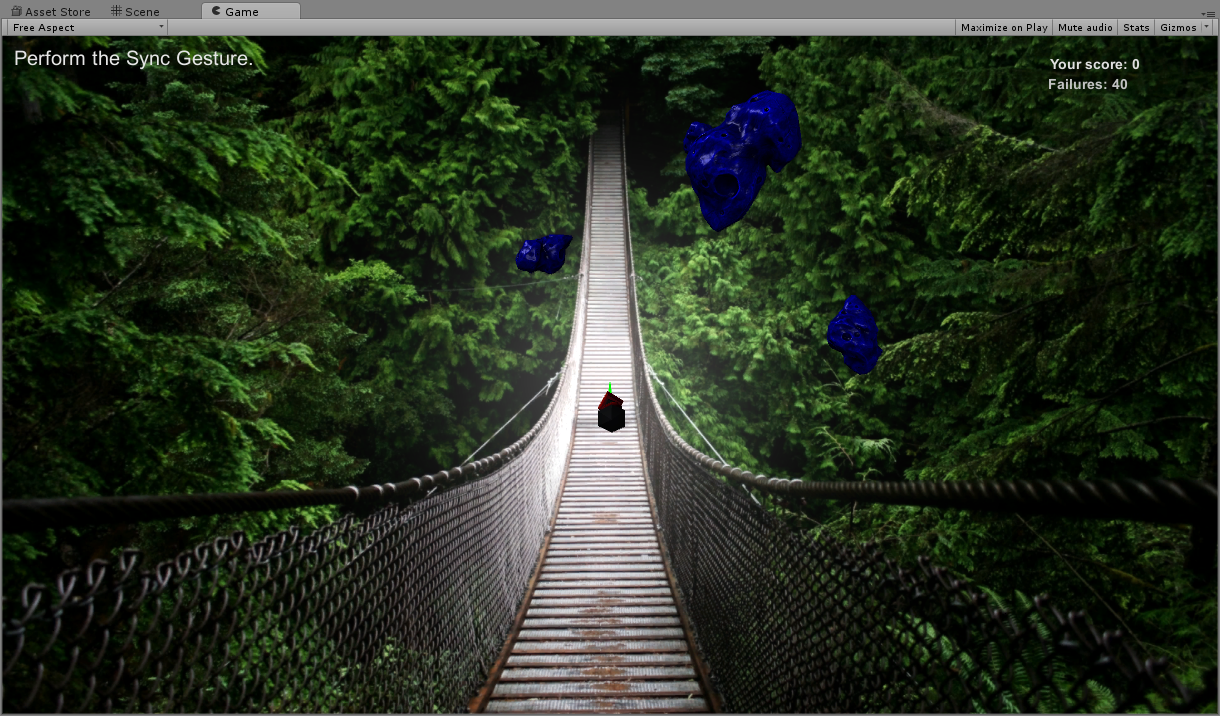
\includegraphics[width=\textwidth]{graphics/screen_v1.png} 
\caption{An alpha version of the game.}
\end{figure}
\subsection{Testing of beta version(children)}


\textbf{State of the game:} The game support controlling with two Myo devices - one for waving the wand and one for casting the spells with gestures. Lasers have better contrast. Asteroids have different colors and reacts only to lasers of appropriate colors. Background is now 3D terrain with skybox. The aim device has been introduced (green sight that gets red if on line with any target). The UI shows available gestures and their colors. Not destroyed asteroids now explode in front of the player. Objects like lasers and asteroids have time-based destructors to avoid the stack overflow. Levelling up mechanism has been implemented.

\textbf{Testing group:} two girls, 9 years old and one adult, without supervision

\textbf{Testing outcome:}

\begin{itemize}
\item aiming mechanism still too hard
\item two hands-based control works fine and even allows cooperative play
\item there are problem with calibrating the device and detecting the gestures
\end{itemize}

\begin{figure}
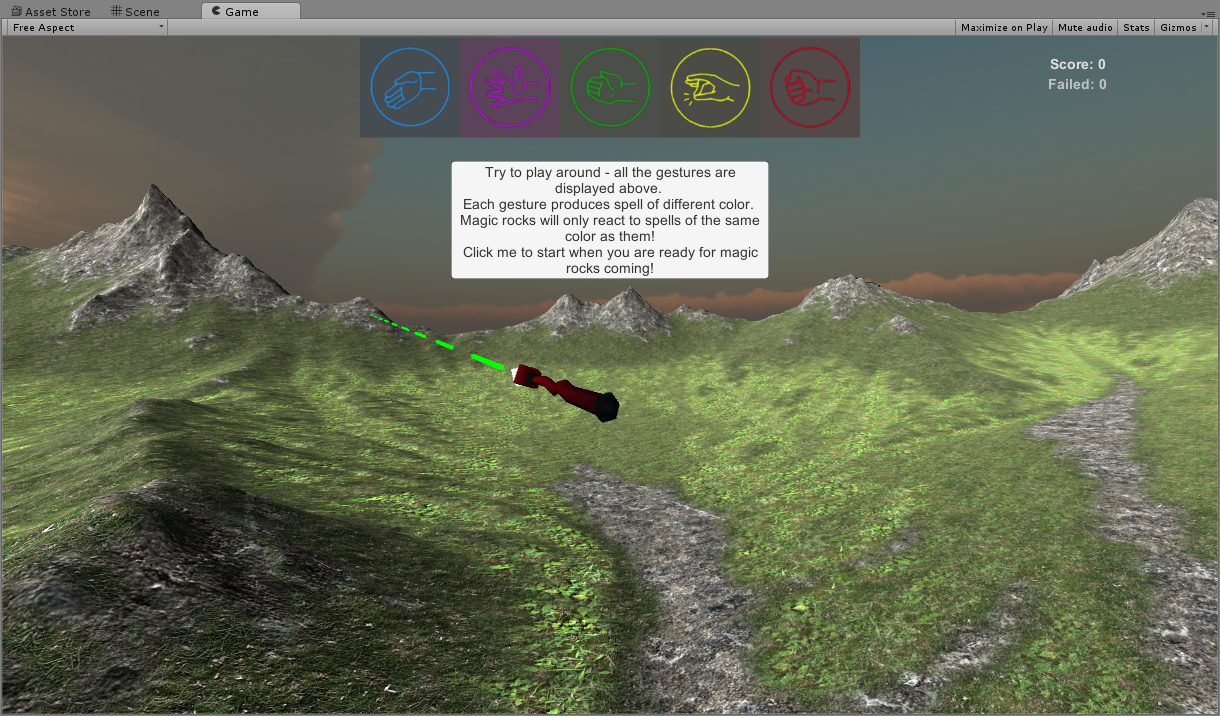
\includegraphics[width=\textwidth]{graphics/screen_v2a.png} 
\caption{A beta version of the game - training screen.}
\end{figure}

\begin{figure}
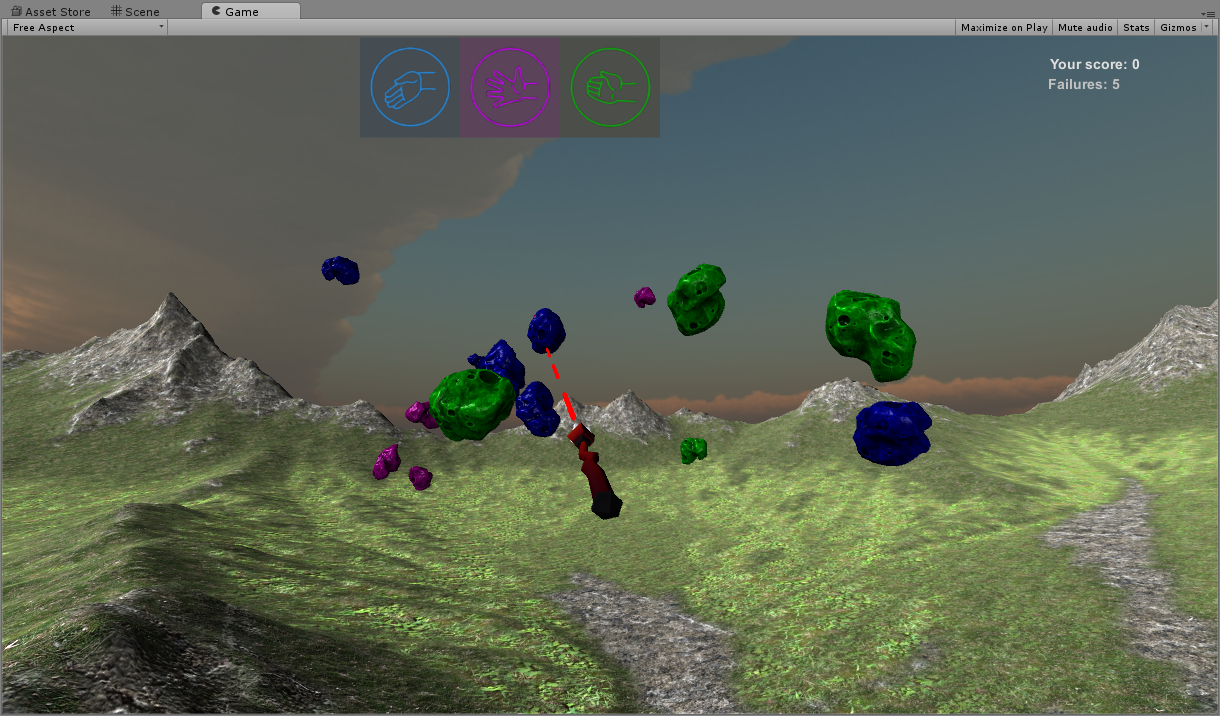
\includegraphics[width=\textwidth]{graphics/screen_v2b.png} 
\caption{A beta version of the game - casual screen view on third level.}
\end{figure}

\subsection{Testing of beta version(adults)}


\textbf{State of the game:} Same as in version for children.


\textbf{Testing group}: 2 males, under 30 yo, with supervision of author

\textbf{Testing outcome:}

\begin{itemize}
\item aiming problem persists
\item some gestures are not recognized as easily as the others
\item game was easily completed in a few minutes
\end{itemize}

